\documentclass[conference]{IEEEtran}
\IEEEoverridecommandlockouts
\usepackage{cite}
\usepackage{amsmath,amssymb,amsfonts}
\usepackage{algorithmic}
\usepackage{graphicx}
\usepackage{textcomp}
\usepackage{xcolor}

\usepackage{booktabs}
\usepackage{multirow}
\usepackage{array}
\def\BibTeX{{\rm B\kern-.05em{\sc i\kern-.025em b}\kern-.08em
    T\kern-.1667em\lower.7ex\hbox{E}\kern-.125emX}}



\begin{document}

\title{Blockchain and IoT Technologies for Secure and Sustainable Urban Management: A Survey}

\author{\IEEEauthorblockN{Nguyen Phuong Linh}
\IEEEauthorblockA{\textit{dept. name of organization (of Aff.)} \\
\textit{name of organization (of Aff.)}\\
City, Country \\
email address}
}

\maketitle


\begin{abstract}
The convergence of blockchain and Internet of Things (IoT) technologies presents transformative opportunities for secure and sustainable urban management. This survey synthesizes findings from three recent studies spanning blockchain based IoT security, blockchain for digital cultural heritage resources (DCHR), and IoT enabled smart parking systems. We analyze how decentralized architectures address persistent challenges in trust management, identity verification, data integrity, and resource optimization across these domains. The survey examines key enabling mechanisms including decentralized identifiers (DIDs), verifiable credentials (VCs), smart contracts, and lightweight consensus protocols. Comparative analysis reveals shared challenges of scalability, regulatory compliance, energy efficiency, and interoperability, alongside domain specific solutions. Results from the reviewed studies demonstrate that IoT based smart parking reduces search time by 42\% and CO2 emissions by 27\%, while blockchain based trust frameworks effectively mitigate Sybil attacks and device spoofing. We identify future research directions including AI blockchain fusion, green consensus algorithms, and cross domain standardization.
\end{abstract}

\begin{IEEEkeywords}
blockchain, Internet of Things, trust management, decentralized identity, smart parking, cultural heritage, smart contracts, sustainability
\end{IEEEkeywords}

\section{Introduction}

The Internet of Things (IoT) ecosystem connects billions of heterogeneous devices ranging from smart home appliances and industrial sensors to healthcare monitors and autonomous vehicles. While this interconnected infrastructure enables unprecedented automation, efficiency, and real time decision making, it simultaneously introduces substantial challenges related to trust, security, identity management, and data integrity~\cite{b1}. These challenges are amplified by the resource constrained nature of IoT devices, their physical exposure, and the dynamic topology of IoT networks.

Traditional centralized trust management approaches, including trusted third parties, centralized reputation systems, and cloud based access control, suffer from single points of failure, scalability limitations, and vulnerability to insider threats~\cite{b1}. Blockchain technology, with its inherent properties of decentralization, immutability, transparency, and cryptographic security, provides a promising foundation for addressing these limitations across diverse application domains~\cite{b2}.

\begin{figure}[htbp]
\centerline{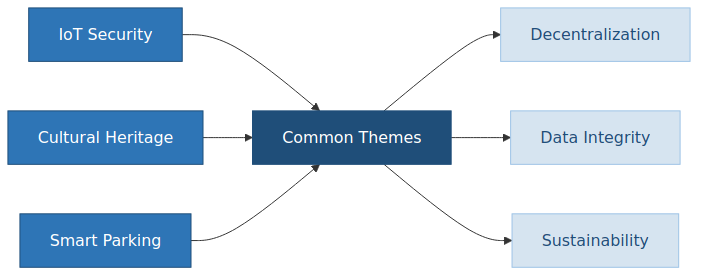
\includegraphics[width=\columnwidth]{images/fig_survey_scope.png}}
\caption{Survey scope: three domains converging on common themes of decentralization, data integrity, transparency, and sustainability.}
\label{fig:scope}
\end{figure}

Beyond security, IoT technologies are increasingly deployed for urban sustainability objectives. Sensor equipped smart parking systems demonstrate measurable improvements in traffic congestion, fuel consumption, and carbon emissions through real time occupancy detection and predictive routing~\cite{b3}. Similarly, blockchain has emerged as a transformative tool for digital cultural heritage preservation, where provenance tracking, authenticity certification, and intellectual property management are paramount concerns~\cite{b2}.

This survey synthesizes findings from three complementary studies: (1) a comprehensive review of blockchain for IoT security covering identity management, access control, and trust mechanisms~\cite{b1}; (2) a review of blockchain technology for digital cultural heritage resources management~\cite{b2}; and (3) a multiagent simulation study of IoT based smart parking for sustainable urban mobility~\cite{b3}. By analyzing these works together, we identify cross domain patterns, shared challenges, and converging future directions at the intersection of blockchain and IoT technologies.

\section{Literature Review}

\subsection{Blockchain for IoT Security}

\begin{figure}[htbp]
\centerline{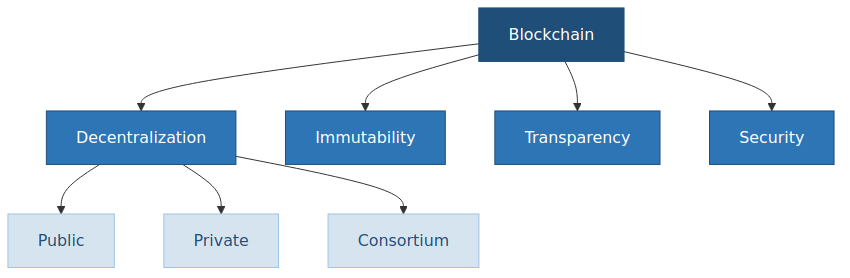
\includegraphics[width=\columnwidth]{images/fig_blockchain_core.png}}
\caption{Core blockchain properties and classification for IoT applications, showing how public, private, and consortium chains serve different security and governance requirements.}
\label{fig:blockchain}
\end{figure}

Khayer et al.~\cite{b1} present a narrative review synthesizing 77 peer reviewed studies (2020--2025) on blockchain based trust management for IoT. Their PRISMA style screening process identified studies from IEEE Xplore, ACM Digital Library, SpringerLink, and MDPI, with quality assessment using a 0--8 rubric (median score: 5/8). The review spans five major domains: industrial IoT (15 studies), smart cities (14), vehicular IoT (12), healthcare (13), and cross domain frameworks (23).

\subsubsection{Trust Management Frameworks}

Blockchain enables decentralized trust evaluation through device behavior analysis, interaction histories, and context aware mechanisms, replacing vulnerable centralized models. Notable approaches include integrating Physical Unclonable Functions (PUFs) with smart contracts for secure device identity~\cite{b4}, Sybil resistant trust models using blockchain based voting~\cite{b5}, and context aware trust modeling incorporating multi dimensional policy enforcement~\cite{b6}. Bhatt and Sandhu~\cite{b7} proposed an Attribute Based Access Control (ABAC) model for cloud enabled IoT, demonstrating fine grained control across smart home and smart parking scenarios.

\begin{figure}[htbp]
\centerline{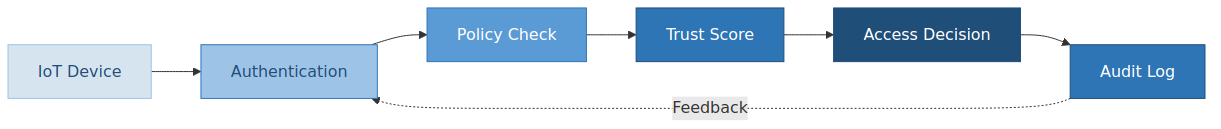
\includegraphics[width=\columnwidth]{images/fig_trust_management.png}}
\caption{Blockchain based trust management framework for IoT showing the flow from device authentication through trust evaluation to access decisions, with inputs from behavioral analysis, reputation scoring, and AI/ML models.}
\label{fig:trust}
\end{figure}

\subsubsection{Decentralized Identity Management}

\begin{figure}[htbp]
\centerline{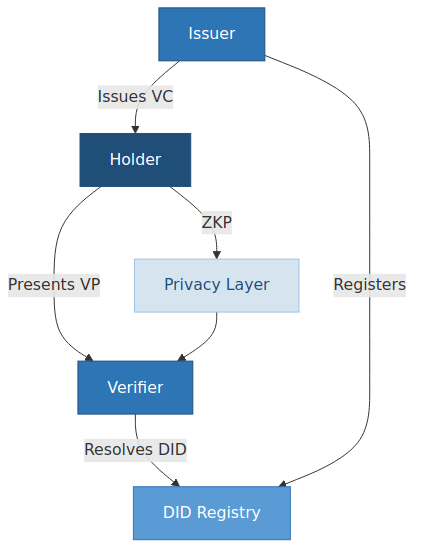
\includegraphics[width=\columnwidth]{images/fig_identity_management.png}}
\caption{Decentralized identity ecosystem showing the interactions among identity holders, credential issuers, and verifiers through DIDs, VCs, and privacy preserving mechanisms including zero knowledge proofs and selective disclosure.}
\label{fig:identity}
\end{figure}

Decentralized Identifiers (DIDs) provide globally unique identifiers controlled directly by the entity without requiring central registries. Dadkhah et al.~\cite{b8} proposed a decentralized IoT onboarding framework for smart homes using consortium blockchain to ensure secure device integration. Ramírez-Gordillo et al.~\cite{b9} introduced a decentralized identity management model using the IOTA Tangle to improve scalability in resource-constrained environments. Verifiable Credentials (VCs) enable selective disclosure of digitally signed credentials; Xu et al.~\cite{b10} designed a privacy-preserving revocation mechanism using cryptographic accumulators to ensure tamper-evident credential management. Self Sovereign Identity (SSI) frameworks such as Hyperledger Indy and uPort grant devices full control over their digital identities~\cite{b11}.

\subsubsection{Consensus Mechanisms for IoT}

\begin{figure}[htbp]
\centerline{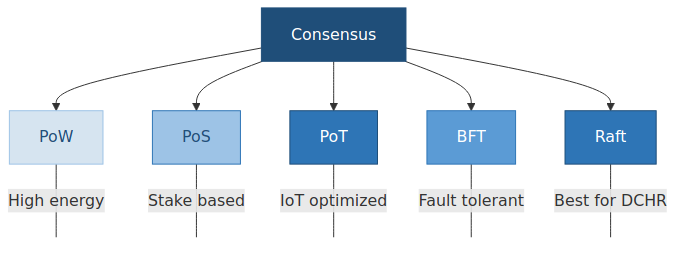
\includegraphics[width=\columnwidth]{images/fig_consensus_comparison.png}}
\caption{Comparison of consensus mechanisms for blockchain IoT networks, evaluating each approach across energy efficiency, throughput, fault tolerance, scalability, and decentralization.}
\label{fig:consensus}
\end{figure}

Traditional Proof of Work (PoW) consensus is impractical for resource constrained IoT devices. Ye et al.~\cite{b12} proposed Proof of Trust (PoT), incorporating device reputation into consensus leader selection to reduce computational redundancy. Liu et al.~\cite{b13} designed hierarchical blockchain architectures distributing consensus between edge and core layers. Hybrid approaches dynamically alternate between BFT and PoT based on node behavior and energy availability~\cite{b14}.

\subsubsection{AI/ML Integration}

AI and machine learning enhance blockchain IoT trust management through behavioral analysis, trust prediction, and anomaly detection. Federated intrusion detection systems integrate deep learning with blockchain for cross node intelligence sharing while preserving data privacy~\cite{b15}. Reinforcement learning enables adaptive smart contract triggers for proactive resource management~\cite{b16}.

\subsection{Blockchain for Digital Cultural Heritage}

\begin{figure}[htbp]
\centerline{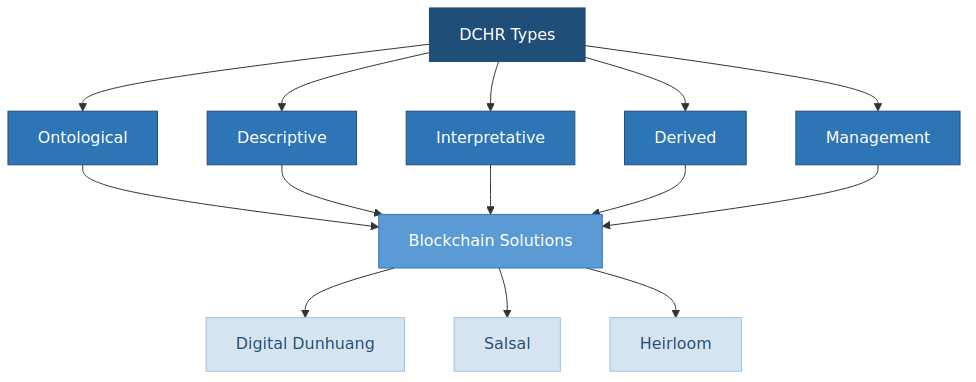
\includegraphics[width=\columnwidth]{images/fig_dchr_taxonomy.png}}
\caption{Digital Cultural Heritage Resources taxonomy with five resource categories, blockchain solutions including NFT tokenization and smart contracts, and implementation cases from Digital Dunhuang to MApp.}
\label{fig:dchr}
\end{figure}

Liu et al.~\cite{b2} review blockchain applications for Digital Cultural Heritage Resources (DCHR), categorizing these resources into ontological, descriptive, interpretative, derived, and management types. Blockchain addresses key challenges in data authentication, privacy protection, copyright management, and equitable resource sharing.

The study evaluates consensus mechanisms specifically for DCHR, finding PoW incompatible due to high energy costs, PoS partially viable for NFT modules, and the Raft algorithm most suitable for centralized DCHR administration due to its fault tolerant leader election and strong consistency guarantees~\cite{b2}. An enhanced Raft algorithm is proposed with improved security through tri phase mechanisms.

Two pivotal case studies demonstrate blockchain's practical impact: the Digital Dunhuang Open Material Library, which reconciles scalability with institutional collaboration through NFT driven economic models, and the Salsal platform, which embeds International Council of Museums ethical guidelines into Ethereum smart contracts for decentralized governance~\cite{b2}. Additional platforms including Heirloom (IPFS based heritage preservation), MApp (minor artwork documentation across Ethereum and Polygon)~\cite{b17}, and BMDRM (NFT driven copyright management) illustrate the breadth of blockchain heritage applications.

The paper raises critical concerns about blockchain potentially establishing ``technocratic authority'' that transfers discursive power to developer communities, and about NFT commodification conflicting with communal ownership norms of indigenous heritage~\cite{b2}.

\subsection{IoT for Smart Urban Mobility}

\begin{figure}[htbp]
\centerline{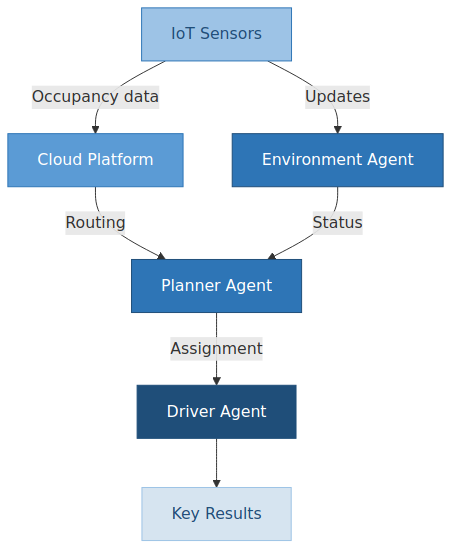
\includegraphics[width=\columnwidth]{images/fig_smart_parking.png}}
\caption{IoT smart parking system architecture showing three agent types (driver, planner, environment), sensor based occupancy detection, cloud analytics, and key performance results.}
\label{fig:parking}
\end{figure}

Mutambik~\cite{b3} constructs a multiagent simulation framework using the Janus platform to evaluate IoT based smart parking. The system employs ultrasonic, magnetic, and infrared sensors for real time occupancy detection, with a predictive guidance module computing optimal routes using real time and historical data.

The simulation models three agent types using Finite State Machine (FSM) transitions: driver agents (idle/navigate/park states), planner agents (coordination and assignment), and environment agents (infrastructure and status updates). Testing across 200--500 parking units with 30 repetitions per scenario over simulated one year periods, the framework evaluates performance across four dimensions~\cite{b3}.

\begin{figure}[htbp]
\centerline{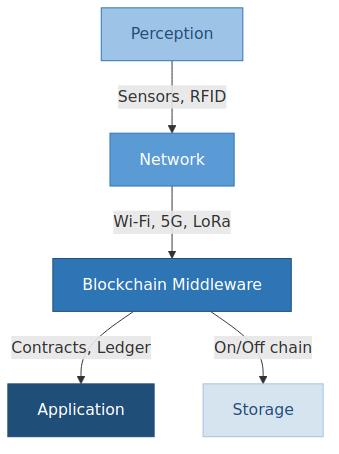
\includegraphics[width=\columnwidth]{images/fig_iot_architecture.png}}
\caption{IoT architecture layers with blockchain integration, spanning perception (sensors), network (communication protocols), middleware (blockchain), application (smart city services), and storage (on chain and off chain).}
\label{fig:arch}
\end{figure}

Results demonstrate substantial improvements: average parking search time decreased by 42\%, congestion within parking zones dropped by 35\%, and CO2 emissions from circling vehicles reduced by 27\%~\cite{b3}. The smart system reduced daily travel distance from approximately 384 km (periodic weekly strategy) to 71 km (smart threshold 0.9), with corresponding CO2 reductions from 309 kg/day to below 75 kg/day.

\section{Analysis and Comparison}

\subsection{Cross Domain Analysis}

\begin{figure}[htbp]
\centerline{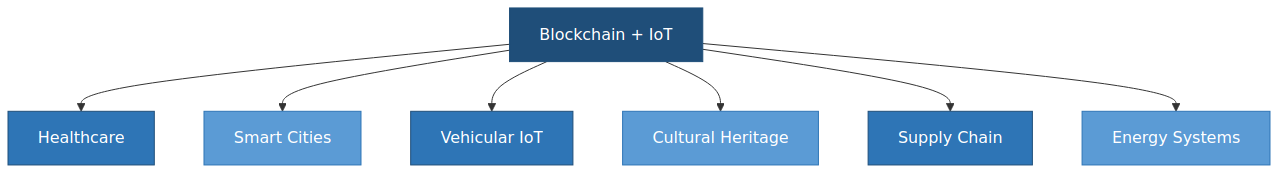
\includegraphics[width=\columnwidth]{images/fig_cross_domain.png}}
\caption{Cross domain applications of blockchain and IoT technologies spanning healthcare, smart cities, vehicular IoT, cultural heritage, supply chain, and energy systems, supported by shared enabling technologies.}
\label{fig:crossdomain}
\end{figure}

Table~\ref{tab:comparison} presents a comparative analysis of the three surveyed studies across key dimensions.

\begin{table*}[htbp]
\caption{Comparative Analysis of Surveyed Studies}
\begin{center}
\begin{tabular}{p{2.5cm}p{4.5cm}p{4.5cm}p{4.5cm}}
\toprule
\textbf{Dimension} & \textbf{Blockchain for IoT Security~\cite{b1}} & \textbf{Blockchain for DCHR~\cite{b2}} & \textbf{IoT Smart Parking~\cite{b3}} \\
\midrule
\textbf{Primary Focus} & Trust, identity, access control & Heritage preservation, provenance & Urban mobility, sustainability \\
\textbf{Blockchain Role} & Decentralized trust and identity & Immutable provenance and rights & Future integration for security \\
\textbf{IoT Role} & Target environment (devices) & Environmental sensing for artifacts & Core sensing infrastructure \\
\textbf{Consensus} & PoT, adaptive PBFT, hybrid & Enhanced Raft, BFT & Not applicable \\
\textbf{Smart Contracts} & Access control, trust updates & Copyright, ethical governance & Not implemented \\
\textbf{Evaluation} & Qualitative survey (77 studies) & Qualitative review (86 refs) & Quantitative simulation \\
\textbf{Validation} & Literature synthesis & Case studies & Agent based simulation \\
\textbf{Key Metrics} & Latency, throughput, energy & Qualitative assessments & Distance, CO2, time, satisfaction \\
\bottomrule
\end{tabular}
\label{tab:comparison}
\end{center}
\end{table*}

\subsection{Shared Challenges and Solutions}

Table~\ref{tab:challenges} maps shared challenges across the three domains to their proposed solutions.

\begin{table}[htbp]
\caption{Shared Challenges Across Domains}
\begin{center}
\begin{tabular}{p{1.8cm}p{6cm}}
\toprule
\textbf{Challenge} & \textbf{Solutions Across Domains} \\
\midrule
Scalability & Hierarchical blockchains~\cite{b13}, edge aggregation, IPFS offloading~\cite{b17}, linear simulation scaling~\cite{b3} \\
\midrule
Energy & PoT consensus~\cite{b12}, enhanced Raft~\cite{b2}, sensor duty cycling~\cite{b3} \\
\midrule
Regulatory & Off chain storage with hash anchoring~\cite{b1}, GDPR compliant consent management~\cite{b18}, cross border sandboxes~\cite{b2} \\
\midrule
Interop. & Standardized DIDs/VCs~\cite{b11}, ERC-1155 cross chain~\cite{b17}, open APIs \\
\midrule
Privacy & Zero knowledge proofs~\cite{b19}, selective disclosure, differential privacy~\cite{b3} \\
\bottomrule
\end{tabular}
\label{tab:challenges}
\end{center}
\end{table}

\subsection{Research Gaps}

Analysis reveals several cross domain research gaps. First, all three studies acknowledge the absence of large scale real world deployments; most blockchain IoT approaches rely on prototypes or simulations. Second, quantitative benchmarking across solutions remains limited; the IoT security survey notes that no study directly compares consensus mechanisms under identical conditions. Third, the economic viability of blockchain deployment, including total cost of ownership and return on investment, is insufficiently explored. Fourth, the smart parking study identifies the need for blockchain integration to secure sensor data transactions, representing a natural convergence point between the IoT security and urban mobility domains.

\section{Conclusion}

\begin{figure}[htbp]
\centerline{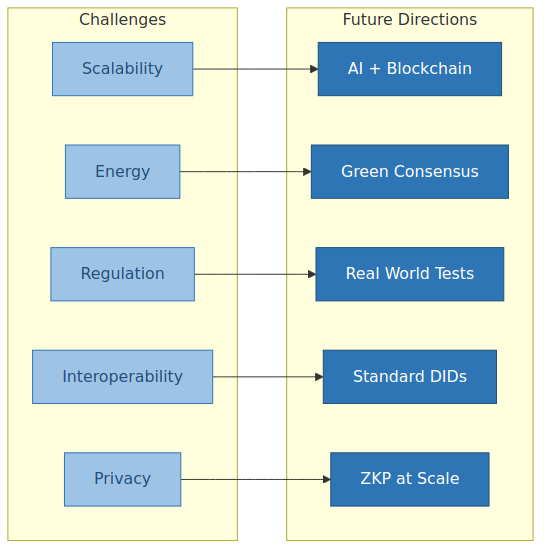
\includegraphics[width=\columnwidth]{images/fig_challenges_future.png}}
\caption{Mapping of current challenges to emerging solutions and future research directions, showing progression from scalability and energy issues toward AI blockchain fusion and green consensus protocols.}
\label{fig:future}
\end{figure}

This survey synthesizes three complementary studies to examine how blockchain and IoT technologies address challenges in security, cultural heritage preservation, and urban sustainability. Our analysis identifies several key findings.

Blockchain provides robust mechanisms for decentralized trust management through DIDs, VCs, and smart contracts, effectively mitigating threats including Sybil attacks, device spoofing, and insider threats in IoT environments. For cultural heritage, blockchain enables immutable provenance tracking, NFT based tokenization, and ethical governance through smart contract encoded institutional guidelines. IoT sensor networks, when combined with predictive analytics, demonstrate measurable sustainability improvements: 42\% reduction in parking search time, 35\% congestion decrease, and 27\% lower CO2 emissions.

Shared challenges across domains include scalability limitations of public blockchains, regulatory tensions between immutability and privacy regulations such as GDPR, energy consumption of traditional consensus mechanisms, and interoperability across heterogeneous systems. Promising solutions include hierarchical blockchain architectures, lightweight consensus protocols such as Proof of Trust, off chain storage patterns, and standardized identity frameworks.

Future research should pursue several converging directions: (1) AI blockchain fusion through federated learning with on chain triggers for privacy preserving intelligence; (2) green consensus algorithms designed for constrained IoT environments; (3) large scale real world validation across diverse urban contexts; (4) cross domain standardization of DID schemas and onboarding protocols; and (5) regulatory frameworks that reconcile decentralized architectures with evolving privacy legislation. The convergence of blockchain and IoT technologies holds substantial promise for building secure, transparent, and sustainable urban management systems, provided that scalability, compliance, and deployment cost barriers are systematically addressed.

\section*{Acknowledgment}

The authors thank the reviewers whose detailed analyses of the three surveyed papers provided the foundation for this comparative study.

\begin{thebibliography}{00}
\bibitem{b1} B. Khayer, S. Mirzaei, H. Alavizadeh, and A. Salehi Shahraki, ``Blockchain for secure IoT: A review of identity management, access control, and trust mechanisms,'' \textit{IoT}, vol. 6, no. 4, p. 65, 2025.
\bibitem{b2} X. Liu, F. Dong, W. Shui, and G. Geng, ``Blockchain technology for digital cultural heritage resources management,'' \textit{npj Heritage Science}, vol. 13, Art. no. 235, 2025.
\bibitem{b3} I. Mutambik, ``Sustainable IoT-enabled parking management: A multiagent simulation framework for smart urban mobility,'' \textit{Sustainability}, vol. 17, no. 14, p. 6382, 2025.
\bibitem{b4} U. Javaid, M. N. Aman, and B. Sikdar, ``Secure blockchain-based IoV architecture integrated with PUFs for secure vehicular communication,'' \textit{IEEE Internet of Things J.}, vol. 7, no. 12, pp. 11338--11349, 2020.
\bibitem{b5} S. Asiri and A. Miri, ``A Sybil resistant IoT trust model using blockchains,'' in \textit{Proc. IEEE Int. Conf. Internet of Things (iThings) GreenCom CPSCom SmartData}, 2018, pp. 1017--1026.
\bibitem{b6} L. Song, Z. Zhu, M. Li, L. Ma, and X. Ju, ``A novel access control for Internet of Things based on blockchain smart contract,'' in \textit{Proc. IEEE 5th Adv. Inf. Technol., Electron. Autom. Control Conf. (IAEAC)}, 2021, pp. 1--5.
\bibitem{b7} S. Bhatt and R. Sandhu, ``ABAC-CC: Attribute-based access control and communication control for Internet of Things,'' \textit{IEEE Access}, vol. 9, 2021.
\bibitem{b8} N. Dadkhah, K. Reaz, and G. Wunder, ``Towards a decentralized IoT onboarding for smart homes using consortium blockchain,'' \textit{arXiv preprint arXiv:2502.13961}, 2025.
\bibitem{b9} T. Ramírez-Gordillo, A. Maciá-Lillo, F. A. Pujol, N. García-D'Urso, J. Azorín-López, and H. Mora, ``Decentralized identity management for Internet of Things (IoT) devices using IOTA blockchain technology,'' \textit{Future Internet}, vol. 17, no. 1, p. 35, 2025.
\bibitem{b10} L. Xu, T. Li, and Z. Erkin, ``Verifiable credentials with privacy-preserving tamper-evident revocation mechanism,'' in \textit{Proc. IEEE 5th Int. Conf. Blockchain Comput. Appl. (BCCA)}, 2023, pp. 1--8.
\bibitem{b11} N. Kulabukhova, A. Bogdanov, and V. Korkhov, ``Evaluating ledger based SSI frameworks for IoT,'' in \textit{Proc. ICCSA}, Springer, 2021, pp. 426--441.
\bibitem{b12} B. Ye, M. Li, and L. Chen, ``A Proof-of-Trust consensus protocol for enhancing accountability in crowdsourcing services,'' \textit{IEEE Trans. Serv. Comput.}, vol. 15, no. 4, pp. 1827--1840, 2022.
\bibitem{b13} D. Liu, J. Ni, and X. Shen, ``Cross domain authentication on hierarchical blockchain for IoT,'' \textit{IEEE Trans. Inf. Forensics Security}, vol. 17, pp. 2861--2875, 2022.
\bibitem{b14} A. Rouzbahani and F. Taghiyareh, ``SCoTMan: A scalable smart contract based trust framework for social IoT,'' \textit{IEEE Access}, vol. 11, pp. 31450--31465, 2023.
\bibitem{b15} F. Al-Turjman, M. H. Zahmatkesh, and R. Shahroze, ``Federated intrusion detection for industrial IoT with blockchain,'' \textit{IEEE Trans. Ind. Inform.}, vol. 18, no. 11, pp. 7978--7989, 2022.
\bibitem{b16} A. Chandan, J. Singh, and P. Raj, ``Adaptive blockchain IoT framework with reinforcement learning,'' \textit{IEEE Access}, vol. 10, pp. 82346--82360, 2022.
\bibitem{b17} F. Valeonti, A. Bikakis, A. Terras, C. Speed, A. Hudson-Smith, and K. Chalkias, ``Crypto collectibles, museum funding and OpenGLAM: Challenges, opportunities and the potential of Non-Fungible Tokens (NFTs),'' \textit{Applied Sciences}, vol. 11, no. 21, p. 9931, 2021.
\bibitem{b18} A. Politou, E. Alepis, and C. Patsakis, ``Forgetting personal data and revoking consent under the GDPR: Challenges and solutions,'' \textit{J. Cybersecur.}, vol. 4, no. 1, 2018.
\bibitem{b19} G. Ramezan and E. Meamari, ``zk-IoT: Securing the Internet of Things with Zero-Knowledge Proofs on blockchain platforms,'' \textit{arXiv preprint arXiv:2402.08322}, 2024.
\end{thebibliography}

\end{document}
